\documentclass[]{article}
\usepackage{amsmath,amsfonts,pstricks,pst-eps,tikz,verbatim,mathtools,graphicx}
\pagestyle{empty}
\title{Final project}
\author{Jiawen Bi}
\allowdisplaybreaks
\date{\today}
\begin{document}
\maketitle


%=============================================================================================================================================================

\section{Preparation and B-spline algorithm}
\par
The whole function is $$
    P(x) = \sum_{i=0}^n P_i B_i^k(x)
   	$$
where $P_i$ is the de Boor point, $B_i^k(x)$ is the basis function according to the handout. 
I am going to use the cubic B-spline curve to fit the pattern.\par
We know according to Example 4.26 that the basis quadratic B-spline $$
	B_i^2(x) = \begin{dcases}
	\frac{(x-t_{i-1})^2}{(t_{i+1}-t_{i-1})(t_i - t_{i-1})} & x\in \left(t_{i-1},t_i\right] \\
	\frac{(x-t_{i-1})(t_{i+1}-x)}{(t_{i+1}-t_{i-1})(t_{i+1}-t_i)} + \frac{(t_{i+2}-x)(x-t_i)}{(t_{i+2}-t_i)(t_{i+1}-t_i)} & x\in \left(t_i,t_{i+1}\right] \\
	\frac{(t_{i+2}-x)^2}{(t_{i+2}-t_i)(t_{i+2}-t_{i+1})} & x\in \left(t_{i+1},t_{i+2} \right] \\
	0 & otherwise
	\end{dcases}
$$
and according to Definition 4.24, $$
	B_i^{n+1}(x) = \frac{x-t_{i-1}}{t_{i+n}-t_{i-1}}B_i^n(x) + \frac{t_{i+n+1} - x}{t_{i+n+1}-t_i} B_{i+1}^n(x)
$$
so we can get the basis cubic B-spline $$
	B_i^3(x) = \begin{dcases}
	\frac{(x-t_{i-1})^3}{(t_{i+2}-t_{i-1})(t_{i+1}-t_{i-1})(t_i-t_{i-1})} & \left(t_{i-1},t_i\right] \\
	\frac{(t_{i+3}-x)(x-t_{i})^2}{(t_{i+3}-t_i)(t_{i+1}-t_{i})(t_{i+2}-t_{i})} + \frac{(x-t_{i-1})^2(t_{i+1}-x)}{(t_{i+2}-t_{i-1})(t_{i+1}-t_{i-1})(t_{i+1}-t_i)} & \cdots \\ 
	 + \frac{(t_{i+2}-x)(x-t_i)(x-t_{i-1})}{(t_{i+2}-t_i)(t_{i+1}-t_i)(t_{i+2}-t_{i-1})} & \left(t_i,t_{i+1} \right] \\
	\frac{(t_{i+2}-x)^2(x-t_{i-1})}{(t_{i+2}-t_{i-1})(t_{i+2}-t_i)(t_{i+2}-t_{i+1})} + \frac{(t_{i+3}-x)(x-t_{i})(t_{i+2}-x)}{(t_{i+3}-t_i)(t_{i+2}-t_{i})(t_{i+2}-t_{i+1})} & \cdots\\
	+\frac{(t_{i+3}-x)^2(x-t_{i+1})}{(t_{i+3}-t_i)(t_{i+3}-t_{i+1})(t_{i+2}-t_{i+1})} & \left(t_{i+1},t_{i+2} \right] \\
	\frac{(t_{i+3}-x)^3}{(t_{i+3}-t_i)(t_{i+3}-t_{i+1})(t_{i+3}-t_{i+2})} & \left(t_{i+2},t_{i+3} \right]
	\end{dcases}
$$
since $\displaystyle P(x) = \sum P_iB_i^3(x) $, thus for every interval$\displaystyle\left(t_{i-1},t_i\right]$,
\begin{align*}
	P(x) &= P_iB_i^3(x) + P_{i-1}B_{i-1}^3 + P_{i-2}B_{i-2}^3 + P_{i-3}B_{i-3}^3 \\
	&= P_i\frac{x^3 - 3t_{i-1}x^2 + 3t_{i-1}^2x - t_{i-1}^3}  {(t_{i+2} - t_{i-1})(t_{i+1} - t_{i-1})(t_i - t_{i-1})} \\
	&+ P_{i-1}\frac{-x^3 + (2t_{i-2}+t_{i+2})x^2 - (t_{i-2}^2+2t_{i-2}t_{i+2})x + t_{i+2}t_{i-2}^2}  {(t_{i+2} - t_{i-1})(t_{i-1} - t_{i-2})(t_i - t_{i-2})} \\
	&+ P_{i-1}\frac{-x^3 + (2t_{i-2}+t_i)x^2 - (t_{i-2}^2+2t_{i-2}t_i)x + t_{i-2}^2t_i}  {(t_{i+1} - t_{i-2})(t_i - t_{i-2})(t_i-t_{i-1})} \\
	&+ P_{i-1}\frac{-x^3 + (t_{i-1}+t_{i+1}+t_{i-2})x^2 - (t_{i-1}t_{i+1}+t_{i-2}t_{i-1}+t_{i-2}t_{i+1})x+t_{i-1}t_{i+1}t_{i-2}}  {(t_{i+1}-t_{i-1})(t_i-t_{i-1})(t_{i-1}-t_{i-2})} \\
	&+ P_{i-2}\frac{x^3 - (2t_i+t_{i-3})x^2 + (t_i^2+2t_it_{i-3})x - t_i^2t_{i-3}}  {(t_i-t_{i-3})(t_i-t_{i-2})(t_i-t_{i-1})} \\
	&+ P_{i-2}\frac{x^3 - (t_{i+1}+t_{i-1}+t_{i-3})x^2 + (t_{i-1}t_{i+1}+t_{i+1}t_{i-3}+t_{i-1}t_{i-3})x - t_{i+1}t_{i-1}t_{i-3}}  {(t_{i-1}-t_{i-3})(t_{i-1}-t_{i-2})(t_i-t_{i-2})} \\
	&+ P_{i-2}\frac{x^3 - (t_i+t_{i+1}+t_{i-2})x^2 + (t_it_{i-1}+t_it_{i-2}+t_{i+1}t_{i-2})x - t_it_{i+1}t_{i-2}}  {(t_{i+1}-t_{i-2})(t_i-t_{i-2})(t_{i-1}-t_{i-2})} \\
	&+ P_{i-3}\frac{-x^3 + (2t_{i-1}+t_i)x^2 - (t_{i-1}^2+2t_it_{i-1})x + t_{i-1}^2t_i}  {(t_i-t_{i-3})(t_{i-1}-t_{i-3})(t_{i-1}-t_{i-2})}
\end{align*}
\begin{comment}
Then $\displaystyle P(x) = [\frac{P_i}{(t_{i+2} - t_{i-1})(t_{i+1} - t_{i-1})(t_i - t_{i-1})} - \frac{P_{i-1}}{(t_{i+2} - t_{i-1})(t_{i-1} - t_{i-2})(t_i - t_{i-2})}\\ 
-\frac{P_{i-1}}{(t_{i+1} - t_{i-2})(t_i - t_{i-2})(t_i-t_{i-1})} - \frac{P_{i-1}}{(t_{i+1}-t_{i-1})(t_i-t_{i-1})(t_{i-1}-t_{i-2})} \\
+ \frac{P_{i-2}}{(t_i-t_{i-3})(t_i-t_{i-2})(t_i-t_{i-1})} + \frac{P_{i-2}}{(t_{i-1}-t_{i-3})(t_{i-1}-t_{i-2})(t_i-t_{i-2})} \\
+ \frac{P_{i-2}}{(t_{i+1}-t_{i-2})(t_i-t_{i-2})(t_{i-1}-t_{i-2})} - \frac{P_{i-3}}{(t_i-t_{i-3})(t_{i-1}-t_{i-3})(t_{i-1}-t_{i-2})}]
\cdot x^3 \\
+ [-\frac{P_i\cdot 3t_{i-1}}{(t_{i+2} - t_{i-1})(t_{i+1} - t_{i-1})(t_i - t_{i-1})}  +  \frac{P_{i-1}(2t_{i-2}+t_{i+2})}{(t_{i+2} - t_{i-1})(t_{i-1} - t_{i-2})(t_i - t_{i-2})}\\
+ \frac{P_{i-1}(2t_{i-2}+t_i)}{(t_{i+1} - t_{i-2})(t_i - t_{i-2})(t_i-t_{i-1})}  +  \frac{P_{i-1}(t_{i-1}+t_{i+1}+t_{i-2})}{(t_{i+1}-t_{i-1})(t_i-t_{i-1})(t_{i-1}-t_{i-2})} \\
- \frac{P_{i-2}(2t_i+t_{i-3})}{(t_i-t_{i-3})(t_i-t_{i-2})(t_i-t_{i-1})}  -  \frac{P_{i-2}(t_{i+1}+t_{i-1}+t_{i-3})}{(t_{i-1}-t_{i-3})(t_{i-1}-t_{i-2})(t_i-t_{i-2})} \\
- \frac{P_{i-2}(t_i+t_{i+1}+t_{i-2})}{(t_{i+1}-t_{i-2})(t_i-t_{i-2})(t_{i-1}-t_{i-2})}  + \frac{P_{i-3}(2t_{i-1}+t_i)}{(t_i-t_{i-3})(t_{i-1}-t_{i-3})(t_{i-1}-t_{i-2})}
]\cdot x^2\\
+ [\frac{P_i(3t_{i-1}^2)}{(t_{i+2} - t_{i-1})(t_{i+1} - t_{i-1})(t_i - t_{i-1})}  -  \frac{P_{i-1}(t_{i-2}^2+2t_{i-2}t_{i+2})}{(t_{i+2} - t_{i-1})(t_{i-1} - t_{i-2})(t_i - t_{i-2})}\\
-\frac{P_{i-1}(t_{i-2}^2+2t_{i-2}t_i)}{(t_{i+1} - t_{i-2})(t_i - t_{i-2})(t_i-t_{i-1})}  -  \frac{P_{i-1}(t_{i-1}t_{i+1}+t_{i-2}t_{i-1}+t_{i-2}t_{i+1})}{(t_{i+1}-t_{i-1})(t_i-t_{i-1})(t_{i-1}-t_{i-2})} \\
+ \frac{P_{i-2}(t_i^2+2t_it_{i-3})}{(t_i-t_{i-3})(t_i-t_{i-2})(t_i-t_{i-1})}  +  \frac{P_{i-2}(t_{i-1}t_{i+1}+t_{i+1}t_{i-3}+t_{i-1}t_{i-3})}{(t_{i-1}-t_{i-3})(t_{i-1}-t_{i-2})(t_i-t_{i-2})} \\
+ \frac{P_{i-2}(t_it_{i-1}+t_it_{i-2}+t_{i+1}t_{i-2})}{(t_{i+1}-t_{i-2})(t_i-t_{i-2})(t_{i-1}-t_{i-2})}  -  \frac{P_{i-3}(t_{i-1}^2+2t_it_{i-1})}{(t_i-t_{i-3})(t_{i-1}-t_{i-3})(t_{i-1}-t_{i-2})}
]\cdot x\\
-\frac{P_it_{i-1}^3}{(t_{i+2} - t_{i-1})(t_{i+1} - t_{i-1})(t_i - t_{i-1})}  +  \frac{P_{i-1}t_{i+2}t_{i-2}^2}{(t_{i+2} - t_{i-1})(t_{i-1} - t_{i-2})(t_i - t_{i-2})}\\
+ \frac{P_{i-1}t_{i-2}^2t_i}{(t_{i+1} - t_{i-2})(t_i - t_{i-2})(t_i-t_{i-1})}  +  \frac{P_{i-1}t_{i-1}t_{i+1}t_{i-2}}{(t_{i+1}-t_{i-1})(t_i-t_{i-1})(t_{i-1}-t_{i-2})} \\
- \frac{P_{i-2}t_i^2t_{i-3}}{(t_i-t_{i-3})(t_i-t_{i-2})(t_i-t_{i-1})}  -  \frac{P_{i-2}t_{i+1}t_{i-1}t_{i-3}}{(t_{i-1}-t_{i-3})(t_{i-1}-t_{i-2})(t_i-t_{i-2})} \\
- \frac{P_{i-2}t_it_{i+1}t_{i-2}}{(t_{i+1}-t_{i-2})(t_i-t_{i-2})(t_{i-1}-t_{i-2})} + \frac{P_{i-3}t_{i-1}^2t_i}{(t_i-t_{i-3})(t_{i-1}-t_{i-3})(t_{i-1}-t_{i-2})}
$\\
,denoted by $P(x) = a_3x^3+a_2x^2+a_1x+a_0 $.
\end{comment}
Applying this equation to $x$ and $y$, we can get the B-spline curve. For more details, please refer to my C++ code.
\par
\begin{figure}[ht]
	\centering
	
\includegraphics[scale = 0.8]{fig.jpg}
	\caption{Peppa Pig}
	\label{fig:fig}
\end{figure}
In this situation, I choose a cartoon picture of Peppa Pig as in Figure 1
and use "grabit"(a mathtool in MATLAB) to pick points and store the points of each curve in "Data000.txt", $\cdots$, "Data014.txt",respectively.


%=============================================================================================================================================================

\section{About the input/output}
\par
My C++ routine will take "Data000.txt", $\cdots$, "Data014.txt" as input, and output a series of B-spline-based polygon
(using 99 extra points generated according to the polynomials of B-spline between every two original points to draw/represent each spline), 
whose filenames are "output000.txt", $\cdots$, "output014.txt".\par
Also, the poset is represented in paticular way in "inclusion.csv". 
In the csv file, I use $inclusion[i][j]$ to show the partial order i.e. the inclusion of Jordan curves as follows:
$$inclusion[i][j] = \begin{dcases}
	1 &, \gamma_i \leq \gamma_j \\
	empty &, i = j \\
	0 &, \gamma_i \not\leq \gamma_j
\end{dcases}$$



%=============================================================================================================================================================

\section{\textit{make} system}



%=============================================================================================================================================================
\section{Hasse diagram}
\tikzset{
	box/.style = {
	circle,
	minimum width = 10pt,
	minimum height = 10pt,
	inner sep = 2.5pt,
	draw = blue,
	fill = red!20
	}
}
According to the poset of splines with the partial order as the inclusion of Jordan curves, 
we can plot the Hasse diagram as below:\\
\begin{tikzpicture}[sibling distance = 40pt]	% Hasse diagram
\node[box] {$\gamma_0^+$}
	child {node[box] {$\gamma_1^-$}
		child {node[box] {$\gamma_2^+$}}
		child {node[box] {$\gamma_3^+$}}
	}
	child {node[box] {$\gamma_5^-$}}
	child {node[box] {$\gamma_6^-$}}
	child {node[box] {$\gamma_4^-$}
		child {node[box] {$\gamma_9^+$}}
		child {node[box] {$\gamma_{10}^+$}}
		child {node[box] {$\gamma_7^+$}
			child {node[box] {$\gamma_{11}^-$}
				child {node[box] {$\gamma_{13}^+$}}
			}
		}
		child {node[box] {$\gamma_8^+$}
			child {node[box] {$\gamma_{12}^-$}
				child {node[box] {$\gamma_{14}^+$}}
			}
		}
	};

\end{tikzpicture}
%\begin{TeXtoEPS}


%=============================================================================================================================================================

\section{Yin set plot}
From the poset, we can easily find the orientation of each curve. 
Let $\gamma_0,\gamma_2,\gamma_3,\gamma_7,\gamma_8,\gamma_9,\gamma_{10},\gamma_{13},\gamma_{14}$ has positive orientation, 
$\gamma_1,\gamma_4,\gamma_5,\gamma_6,\gamma_{11},\gamma{12}$ has negative orientation, and
let $\mathcal{F}_1 = \left\{ \gamma_0^+,\gamma_1^-,\gamma_4^-,\gamma_5^-,\gamma_6^- \right\} $,
$\mathcal{F}_2 = \left\{ \gamma_7^+,\gamma_8^+,\gamma_{11}^-,\gamma_{12}^- \right\}$,
$\mathcal{F}_3 = \left\{\gamma_2^+\right\} $,$\mathcal{F}_4 = \left\{\gamma_3^+\right\} $,
$\mathcal{F}_5 = \left\{\gamma_9^+\right\} $,$\mathcal{F}_6 = \left\{\gamma_{10}^+\right\} $,
$\mathcal{F}_7 = \left\{\gamma_{13}^+\right\} $,$\mathcal{F}_8 = \left\{\gamma_{14}^+\right\} $\\
 and $\mathcal{F} = \bigcup \mathcal{F}_k $. Then $\rho(\mathcal{F}) = \mathcal{Y} $, and the Yin set is plotted as follows:\\


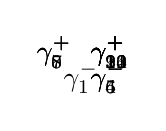
\begin{tikzpicture}
	\draw[draw = red,fill = red!20,scale = 0.04]  plot file {plots/output000.txt}	node[left]{$\gamma_0^+$};
	\draw[draw = red,fill = white,scale = 0.04]  plot file {plots/output001.txt}	node[below]{$\gamma_1^-$};
	\draw[draw = red,fill = red!20,scale = 0.04]  plot file {plots/output002.txt}	node[right]{$\gamma_2^+$};
	\draw[draw = red,fill = red!20,scale = 0.04]  plot file {plots/output003.txt}	node[right]{$\gamma_3^+$};
	\draw[draw = red,fill = white,scale = 0.04]  plot file {plots/output004.txt}	node[below right]{$\gamma_4^-$};
	\draw[draw = red,fill = white,scale = 0.04]  plot file {plots/output005.txt}	node[below right]{$\gamma_5^-$};
	\draw[draw = red,fill = white,scale = 0.04]  plot file {plots/output006.txt}	node[below right]{$\gamma_6^-$};
	\draw[draw = red,fill = red!20,scale = 0.04]  plot file {plots/output007.txt}	node[left]{$\gamma_7^+$};
	\draw[draw = red,fill = red!20,scale = 0.04]  plot file {plots/output008.txt}	node[left]{$\gamma_8^+$};
	\draw[draw = red,fill = red!20,scale = 0.04]  plot file {plots/output009.txt}	node[right]{$\gamma_9^+$};
	\draw[draw = red,fill = red!20,scale = 0.04]  plot file {plots/output010.txt}	node[right]{$\gamma_{10}^+$};
	\draw[draw = red,fill = white,scale = 0.04]  plot file {plots/output011.txt}	node[right]{$\gamma_{11}^-$};
	\draw[draw = red,fill = white,scale = 0.04]  plot file {plots/output012.txt}	node[right]{$\gamma_{12}^-$};
	\draw[draw = red,fill = red!20,scale = 0.04]  plot file {plots/output013.txt}	node[right]{$\gamma_{13}^+$};
	\draw[draw = red,fill = red!20,scale = 0.04]  plot file {plots/output014.txt}	node[right]{$\gamma_{14}^+$};
\end{tikzpicture}
%\end{TeXtoEPS}


\end{document}

